\beginsong{Drei Rote Pfiffe}[
    txt={Heinz Rudolf Unger}, 
    mel={Georg Herrnstadt, Wilhelm Resetarits},
    jahr={1979}, 
    bo={198}, 
    siru={124}, 
    index={Im Kreis ihrer Enkel},
]

\beginverse
\endverse
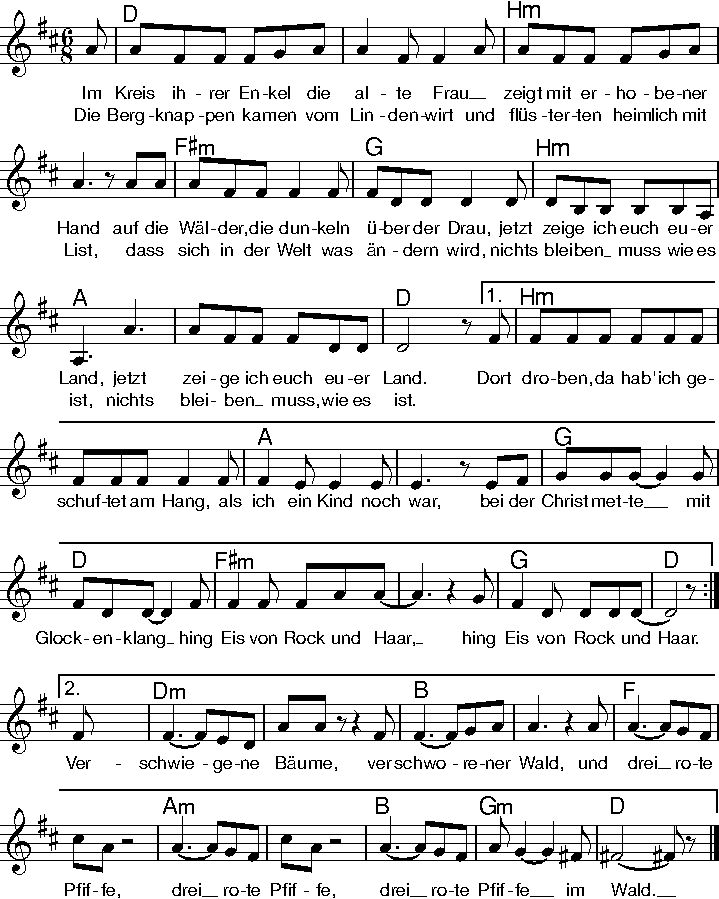
\includegraphics[draft=false, width=1\textwidth]{Noten/Lied030.pdf}	

\beginverse
Die \[D]Drau hinunter trieb Mond um Mond, es \[Hm]brach der Faschistenkrieg aus.
Da \[F#m]hatte ich einen \[G]Mann an der Front 
und \[Hm]hatte drei Kinder im \[A]Haus, und hatte drei Kinder im \[D]Haus.

Wie \[Hm]tönte da markiger Nazigesang von \[A]deutschem Boden und Blut. 
\[G]Manch ein Bursch' in die \[D]Berge entsprang, 
ich trug \[F#m]Flugblätter unter dem Hut, ich trug \[G]Flugblätter unter dem \[D]Hut.

Der \[D]Gestapo war kalt und der Gauleiter schalt: Parti\[Hm]sanen im eigenen Land!
Ich \[F#m]trug das Geflüster und \[G]Brot in den Wald. 
Sie \[Hm]haben mich Jelka ge\[A]nannt. Sie haben mich Jelka ge\[D]nannt.
\endverse

\beginchorus
Ver\[Dm]schwiegene Bäume, ver\[B&]schworener Wald
Und \[F]drei rote Pfiffe, \[Am]drei rote Pfiffe, \[B&]drei rote \[Gm]Pfiffe im \[D]Wald.
\endchorus

\beginverse
Der ^Winter war nass und uns wärmte der Hass, viele ^sind's, die die Erde heut' birgt.
Wir ^haben gefochten, dort ^oben am Pass, 
an ^uns'rer Befreiung ge^wirkt, an uns'rer Befreiung ge^wirkt.

Der ^Krieg war vorbei, da war Stille im Land, da ^waren die Lautesten leis'.
Sie ^nahmen das Hitler^bild von der Wand, 
ihre ^Westen, die wuschen sie weiß, ihre ^Westen, die wuschen sie ^weiß.

^Ihr, meine Enkel, was hört ihr so stumm die ^alten, die kalten Berichte?
Jetzt ^trampeln sie wieder auf euren ^Rechten herum, 
er^innert euch meiner Ge^schichte, erinnert euch meiner Ge^schichte.
\endverse

% \printchorus

\endsong
